% http://tex.stackexchange.com/questions/175671/how-to-use-arara-with-texshop
% !TEX TS-program = arara
% arara: xelatex
% arara: biber
% arara: nomencl
% arara: xelatex: { synctex: yes }
% arara: indent: { overwrite: yes, trace: yes  }
% arara: clean: {files: [basic-mol-evo.aux, basic-mol-evo.idx, basic-mol-evo.ilg, basic-mol-evo.ind, basic-mol-evo.log, basic-mol-evo.bbl, basic-mol-evo.bcf, basic-mol-evo.ist, basic-mol-evo.blg, basic-mol-evo.run.xml, basic-mol-evo.nlo, basic-mol-evo.nls]}

\documentclass[12pt]{article}


\usepackage[a4paper, top=1in, bottom=1.25in, left=1in, right=1in]{geometry}

\usepackage{amssymb,amsmath}
\usepackage{upgreek} % upright greek symbols

% xetex 西文字体
% https://www.reddit.com/r/typography/comments/2vzkad/a_good_serif_webfont_to_pair_with_fira_sans_thats/
\usepackage{fontspec,xltxtra,xunicode}
    \setmainfont[BoldFont={Charter Bold}, ItalicFont={Charter Italic}]{Charter}
    \setmonofont{Fira Mono}

% 中文字体
\usepackage{xeCJK}
    \setCJKmainfont[BoldFont={Songti SC Bold}, ItalicFont={Kaiti SC Regular}]{Songti SC Regular}
    \xeCJKsetup{CJKecglue = {\hskip 0pt plus 0.08\baselineskip}, xCJKecglue = {false}}
    \punctstyle{plain}

% don't move this line above
\defaultfontfeatures{Mapping=tex-text,Scale=MatchLowercase}

% Line spacing
\linespread{1.5}

% make inline codes smaller
%\renewenvironment{texttt}{\small}{}
\renewcommand{\texttt}[1]{{\small\ttfamily #1}}

% use upquote if available, for straight quotes in verbatim environments
\IfFileExists{upquote.sty}{\usepackage{upquote}}{}
% use microtype if available
\IfFileExists{microtype.sty}{%
    \usepackage{microtype}
    \UseMicrotypeSet[protrusion]{basicmath} % disable protrusion for tt fonts
    }{}

% citations
% https://www.sharelatex.com/learn/Biblatex_citation_styles
\usepackage[
    backend=biber,
    style=chicago-authordate,
    url=false,
    doi=false,
    isbn=false,
    maxcitenames=2,
    maxbibnames=40,
    abbreviate=true
]{biblatex}
\addbibresource{popgen.bib}
% http://tex.stackexchange.com/questions/150710/ignore-a-bibliography-field-e-g-urldate-for-eliminating-of-biblatex-biber-w
\DeclareSourcemap{
    \maps[datatype=bibtex]{
        \map[overwrite=true]{
            \step[fieldset=urldate, null]
            \step[fieldset=language, null]
            \step[fieldset=month, null]
            \step[fieldset=day, null]
        }
    }
}

\usepackage[unicode=true]{hyperref}
\urlstyle{same}  % don't use monospace font for urls

\usepackage{graphicx,grffile}
\makeatletter
\def\maxwidth{\ifdim\Gin@nat@width>\linewidth\linewidth\else\Gin@nat@width\fi}
\def\maxheight{\ifdim\Gin@nat@height>\textheight\textheight\else\Gin@nat@height\fi}
\makeatother
% Scale images if necessary, so that they will not overflow the page
% margins by default, and it is still possible to overwrite the defaults
% using explicit options in \includegraphics[width, height, ...]{}
\setkeys{Gin}{width=\maxwidth,height=\maxheight,keepaspectratio}

\usepackage{parskip}
\setlength{\parindent}{2em}
\setlength{\emergencystretch}{3em}  % prevent overfull lines
\providecommand{\tightlist}{%
    \setlength{\itemsep}{0pt}\setlength{\parskip}{0pt}}
%\setcounter{secnumdepth}{0} % will prevent numbering for sections

% Redefines (sub)paragraphs to behave more like sections
\ifx\paragraph\undefined\else
    \let\oldparagraph\paragraph
    \renewcommand{\paragraph}[1]{\oldparagraph{#1}\mbox{}}
\fi
\ifx\subparagraph\undefined\else
    \let\oldsubparagraph\subparagraph
    \renewcommand{\subparagraph}[1]{\oldsubparagraph{#1}\mbox{}}
\fi

% set default figure placement to htbp
\makeatletter
\def\fps@figure{htbp}
\makeatother

%%% custom settings

% subcaption
% http://tex.stackexchange.com/questions/125579/subcaption-with-beamer
\usepackage[compatibility=false]{caption}
\usepackage{subcaption}

% chemistry
\usepackage[version=3]{mhchem}

\usepackage{nomencl}
\makenomenclature

\usepackage{etoolbox}

% Itemize left margin
\usepackage{enumitem}

\usepackage{tikz}
\usetikzlibrary{arrows,positioning,calc,decorations.pathreplacing,decorations.pathmorphing}


\title{分子进化}
\author{王强}
\providecommand{\institute}[1]{}
\institute{南京大学生命科学学院}
\date{\today}

%%% document starts here

\begin{document}

\maketitle

{
    \setcounter{tocdepth}{3}
    \renewcommand\contentsname{目录}
    \tableofcontents
    \newpage
}

\section{中性理论}

分子进化的研究对象是生物大分子 DNA, RNA 和蛋白质的序列, 目的是阐明序列随时间变化或恒定的原因与过程.
下面将介绍许分子进化中, 常用的零假设和替代假设背后的概念基础.

中性理论是分子进化中最广泛使用的零假设的基础.
中性理论的观点是, 大多数突变没有或很少有适应性的优点或缺点, 在选择上是中性的.
因此,遗传漂变是决定突变的命运 (固定或丢失) 的主要进化过程.
在二十世纪五六十年代, 人们普遍认为大多数突变会有实质的适应性差异, 因此大多数突变的命运是由自然选择决定的.
而木村资生 (图 \ref{fig:1}) 认为, 突变和遗传漂变的相互作用可以解释生物群体中的许多遗传变异模式,
以及蛋白质和 DNA 序列的进化 \parencite{kimura1969, kimura1983}.
中性理论的零假设有两个主要预测:
一是物种内群体中样本序列的多态性; 另一个是不同物种间的样本序列之间的差异度.

\begin{figure}
    \center
    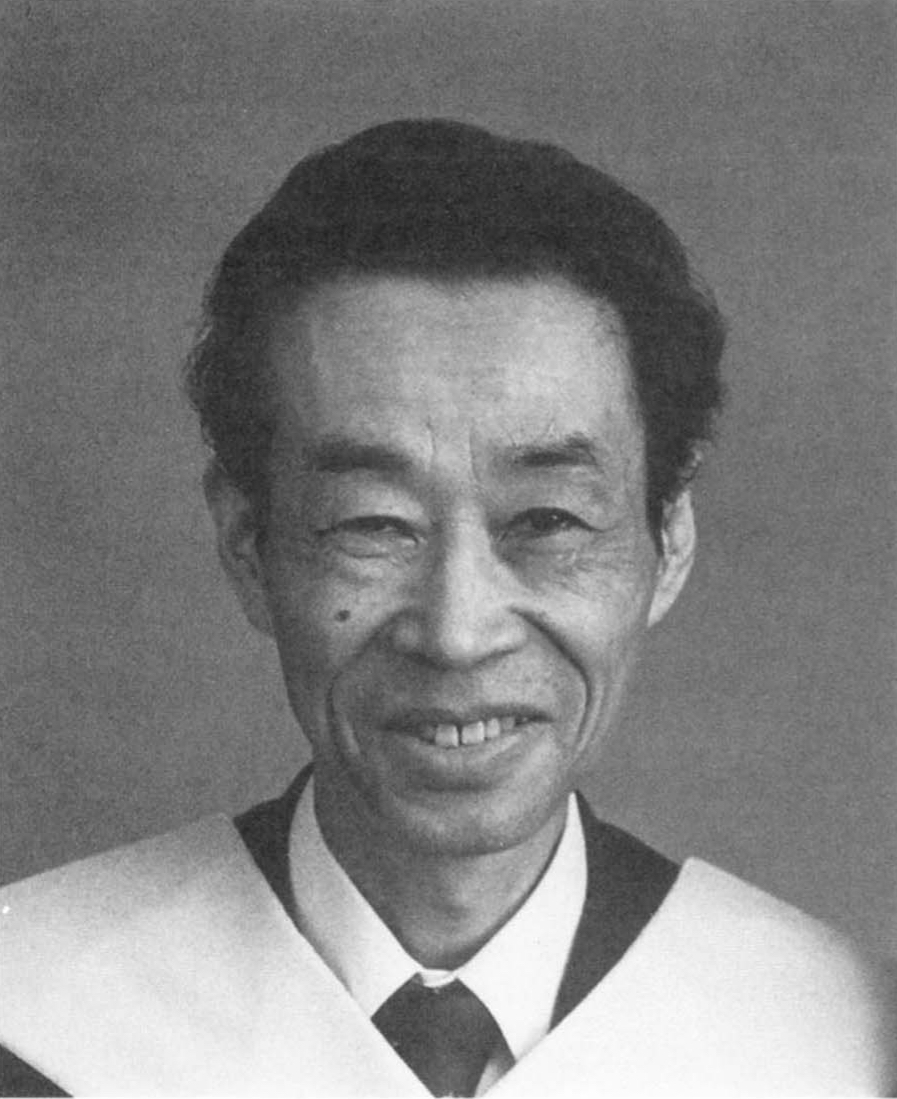
\includegraphics[width=0.5\linewidth]{basic-mol-evo.images/Kimura.jpg}
    \caption{木村资生, Motoo Kimura, 1924--1994. 引自 \textcite{crow1995}.}
    \label{fig:1}
\end{figure}

\subsection{多态性}

\begin{figure}
    \center
    \begin{tikzpicture}[scale=0.5]
        \tikzset{
            drift/.style={
                draw=none,
                postaction={draw=gray,decorate,decoration={segment length=6pt,amplitude=2pt,meta-amplitude=6pt,#1}}
            }
        }
        \draw[help lines] (0,0) grid (30,10);
        \draw[ultra thick, black] (0,0) to (30,0);
        \draw[ultra thick, black] (0,0) to (0,11);
        \node[below =2mm of {(0,0)}] () {$0$};
        \node[below left=2mm of {(30,0)}] () {$t$};
        \node[left =2mm of {(0,0)}] () {$0.0$};
        \node[left =2mm of {(0,10)}] () {$1.0$};
        \node[label={[label distance=4mm,text depth=-1ex,rotate=0]below:Time}] at (15,0) {};
        \node[label={[label distance=4mm,text depth=-1ex,rotate=90]Allel freq.}] at (0,5) {};
        \draw[thick, drift=random steps]
        (0.1,0)
        .. controls (2,2) ..
        (3,0);
        \draw[thick, drift=random steps]
        (1,0)
        .. controls (4,6) ..
        (7,0);
        \draw[ultra thick, drift=random steps, dashed]
        (1.2,0)
        .. controls (4,6) ..
        (7,7)
        .. controls (8,8) ..
        (9,10);
    \end{tikzpicture}
    \caption{The fate of selectively neutral mutations in a population.}
    \label{fig:2}
\end{figure}

\subsection{差异度}

\section{度量差异度与多态性}

\subsection{物种间的 DNA 差异度}

\subsection{DNA 多态性}

\section{DNA 序列差异与分子钟}

\section{检验中性理论的零假设}

\subsection{HKA 检验}

\subsection{MK 检验}

\subsection{Tajima’s D}

\section{非独立位点的分子进化}

\subsection{搭乘效应}

\subsection{连锁不平衡}

\end{document}
